\documentclass[12pt,a4paper]{report}

% ==============================================================================
% PACKAGES & CONFIGURATION
% ==============================================================================
\usepackage[utf8]{inputenc}
\usepackage[T1]{fontenc}
\usepackage{lmodern}
\usepackage[margin=25mm,top=25mm,bottom=25mm]{geometry}
\usepackage{graphicx}
\usepackage{xcolor}
\usepackage{amsmath,amssymb}
\usepackage{tabularx}
\usepackage{booktabs}
\usepackage{array}
\usepackage{fancyhdr}
\usepackage{listings}
\usepackage{tikz}
\usetikzlibrary{shapes.geometric, arrows, positioning, fit, backgrounds, calc}
\usepackage[hidelinks,colorlinks=true,linkcolor=ThaparNavy,urlcolor=ThaparCrimson,citecolor=ThaparNavy]{hyperref}

% Institutional Colors (Thapar Palette)
\definecolor{ThaparCrimson}{RGB}{128, 0, 0}
\definecolor{ThaparNavy}{RGB}{0, 45, 98}
\definecolor{ThaparDark}{RGB}{30, 41, 59}
\definecolor{CodeBg}{RGB}{248, 250, 252}
\definecolor{CodeBorder}{RGB}{226, 232, 240}
\definecolor{BoxBg}{RGB}{248, 249, 252}

% Code Listing Configuration
\lstset{
    language=Java,
    backgroundcolor=\color{CodeBg},
    basicstyle=\ttfamily\footnotesize,
    keywordstyle=\color{ThaparCrimson}\bfseries,
    stringstyle=\color{teal},
    commentstyle=\color{gray}\itshape,
    numbers=left,
    numberstyle=\tiny\color{gray},
    stepnumber=1,
    numbersep=8pt,
    tabsize=4,
    showspaces=false,
    showstringspaces=false,
    breaklines=true,
    breakatwhitespace=true,
    frame=single,
    rulecolor=\color{CodeBorder},
    captionpos=b,
    xleftmargin=15pt,
    framexleftmargin=15pt
}

% Header and Footer Setup
\pagestyle{fancy}
\fancyhf{}
\fancyhead[L]{\small\color{gray}UCS553: Enterprise Web Application}
\fancyhead[R]{\small\color{gray}Syllabix Academic Platform}
\fancyfoot[C]{\thepage}
\renewcommand{\headrulewidth}{0.4pt}
\renewcommand{\footrulewidth}{0.4pt}

% ==============================================================================
% DOCUMENT BEGINS
% ==============================================================================
\begin{document}

% ------------------------------------------------------------------------------
% PAGE 1: OFFICIAL COVER PAGE (Identical to Department Template)
% ------------------------------------------------------------------------------
\begin{titlepage}
\thispagestyle{empty}
\begin{tikzpicture}[remember picture, overlay]
    \draw[line width=2pt, color=black] 
        ($(current page.north west) + (18mm,-18mm)$) 
        rectangle 
        ($(current page.south east) + (-18mm,18mm)$);
\end{tikzpicture}

\begin{center}
    \vspace*{0.2cm}
    {\fontsize{22pt}{26pt}\selectfont \textbf{UCS553: Enterprise Web Application}}\\[0.25cm]
    {\fontsize{18pt}{22pt}\selectfont \textbf{Mini Project Report}}\\[0.9cm]

    {\fontsize{17pt}{22pt}\selectfont \textbf{\color{ThaparCrimson} SYLLABIX: INTELLIGENT STUDENT MANAGEMENT \&\\ADAPTIVE ACADEMIC PLANNING PLATFORM}}\\[1.0cm]

    {\large \textit{Under the Guidance of}}\\[0.2cm]
    {\large \textbf{Dr. ABC, XYZ}}\\[0.1cm]
    {\normalsize Assistant Professor}\\[0.1cm]
    {\normalsize Thapar Institute of Engineering Technology}\\[0.8cm]

    % TI Emblem
    \begin{tikzpicture}
        \node[scale=1.0] at (0,0) {
            \begin{tikzpicture}
                \node[scale=2.2, font=\bfseries\sffamily, text=ThaparCrimson] at (0,0.2) {ti};
                \node[font=\bfseries\sffamily\scriptsize, text=ThaparCrimson, letter space=10] at (0,-0.35) {THAPAR INSTITUTE};
                \node[font=\sffamily\tiny, text=gray] at (0,-0.6) {OF ENGINEERING \& TECHNOLOGY};
                \node[font=\sffamily\tiny\itshape, text=gray] at (0,-0.8) {(Deemed to be University)};
            \end{tikzpicture}
        };
    \end{tikzpicture}\\[0.9cm]

    \begin{flushleft}
    \hspace*{2.2cm}\textbf{\large Submitted By :}\\[0.3cm]
    \hspace*{2.2cm}\begin{tabular}{ll}
        \textbf{Roll Number} & \textbf{Student Name}\\[0.15cm]
        102203045 & Jasmine Kaur
    \end{tabular}
    \end{flushleft}

    \vfill

    {\textbf{\large Computer Science Engineering Department Thapar\\Institute of Engineering Technology, Patiala}}\\[0.4cm]
    {\normalsize \textit{In Partial Fulfilment of the Requirements for the Degree of}}\\[0.1cm]
    {\textbf{Bachelor of Engineering in Computer Engineering}}\\[0.15cm]
    {\normalsize at}\\[0.15cm]
    {\textbf{Thapar Institute of Engineering Technology, Patiala}}\\[0.5cm]
    {\textbf{\large November 2026}}
\end{center}
\end{titlepage}

% ------------------------------------------------------------------------------
% PAGE 2: PROJECT REPORT STRUCTURE & ABSTRACT
% ------------------------------------------------------------------------------
\newpage
\setcounter{page}{2}

\section*{\color{ThaparCrimson} 1. Project Report Structure}

\noindent The following is the updated and simplified report structure adhering to university specifications.

\vspace{0.3cm}
\begin{table}[h!]
\centering
\begin{tabularx}{\textwidth}{|c|X|X|}
\hline
\rowcolor{CodeBorder}
\textbf{S. No.} & \textbf{Section} & \textbf{Contents} \\ \hline
1 & \textbf{Cover Page} & Project title, student names, roll numbers, department and institution \\ \hline
2 & \textbf{Abstract} & Brief overview of the project \\ \hline
3 & \textbf{Table of Contents} & Chapters and page numbers \\ \hline
4 & \textbf{Chapter 1: Introduction} & Project background, problem statement, objectives and scope \\ \hline
5 & \textbf{Chapter 2: System Design} & System architecture, UML diagrams and database design \\ \hline
6 & \textbf{Chapter 3: Implementation} & Technologies, project structure, classes and modules \\ \hline
7 & \textbf{Chapter 4: Results and Screenshots} & Application outputs and screenshots \\ \hline
8 & \textbf{References} & Books, websites and documentation \\ \hline
\end{tabularx}
\end{table}

\vspace{0.4cm}
\section*{\color{ThaparCrimson} Abstract}

Modern higher education institutions present students with complex, fragmented academic environments. At institutions like Thapar Institute of Engineering \& Technology (TIET), a student in their third year balances 7 demanding core courses (e.g., Computer Architecture, Enterprise Web Applications, Machine Learning, Foundations of Data Science, Image Processing, Ethics, and Software Engineering), multiple concurrent continuous assessment components (quizzes, lab evaluations, Mid-Semester Tests, and End-Semester Tests), and tight academic deadlines. Conventional Learning Management Systems (LMS) and college ERP portals act merely as passive repositories—hosting course syllabi as unstructured text or PDF links without providing active guidance. Consequently, students struggle with three critical questions: \textit{(1) What should I study today? (2) When should I study it? (3) Which topics require immediate attention to reach my target grade?}

\textbf{Syllabix} is an intelligent, full-stack student management and adaptive academic planning platform built from the ground up to solve this challenge. Implemented strictly in \textbf{Java 21 / Spring Boot 3.3.5}, Syllabix replaces static CRUD dashboards with an active academic engine. Its flagship features include:
\begin{itemize}
    \item \textbf{Adaptive Study Recommendation Engine:} A normalized, 4-factor weighted heuristic algorithm (35\% Exam Urgency, 30\% Syllabus Incompletion, 20\% Topic Difficulty, 15\% Academic Marks Deficit) that calculates dynamic daily study directives without exceeding declared student availability.
    \item \textbf{Thapar LMS Course Evaluation Scheme Auto-Parser \& Target Run-Rate Calculator:} An intelligent regex parser that extracts assessment components copied directly from Thapar LMS (e.g., MST 30 marks, EST 40 marks, Lab 20 marks, Sessional Quiz 10 marks), tallies completed scores, calculates the exact percentage run-rate needed on remaining evaluations to secure target letter grades ($A^+ \ge 88\%$, $A \ge 80\%$, $B \ge 65\%$), and auto-schedules the milestone assessments.
    \item \textbf{Official Thapar 20-Week Academic Calendar \& Datesheet Tracker:} Direct integration of TIET's ODD SEM 2026-27 schedule, auto-detecting the current week (Week 17 $\bullet$ Teaching), countdowns to Assessment Week (Week 18) and End-Semester Examinations (Weeks 19–20), compensatory Saturday teaching schedules, and gazetted university holidays.
    \item \textbf{Lab Assignment Tracker (Assignments 1 to 8):} Continuous tracking of practical submissions and viva readiness.
    \item \textbf{PDF Syllabus Extractor:} Apache PDFBox-powered text extraction with human-in-the-loop validation for rapid curriculum onboarding.
    \item \textbf{Focus Pomodoro \& Productivity Tracker:} Interval-based study sessions with Web Audio chime synthesis and persistent habit streak tracking.
\end{itemize}

The system is deployed live on the cloud via Docker at \href{https://syllabix-platform-2.onrender.com}{\textbf{https://syllabix-platform-2.onrender.com}} and backed by a comprehensive JUnit 5 and Mockito test suite achieving 100\% pass rates across all core algorithmic services.

% ------------------------------------------------------------------------------
% PAGE 3: TABLE OF CONTENTS
% ------------------------------------------------------------------------------
\newpage
\tableofcontents

% ------------------------------------------------------------------------------
% CHAPTER 1: INTRODUCTION
% ------------------------------------------------------------------------------
\newpage
\chapter{\color{ThaparCrimson} Introduction}

\section{1.1 Introduction to the Project}
In contemporary university education, students are challenged not by a lack of study resources, but by cognitive overload and suboptimal time allocation. University portals provide students with syllabi, datesheets, and evaluation breakdowns, but leave the translation of this raw data into an actionable daily study schedule entirely to the student. Most students resort to ad-hoc, reactive studying—focusing on whichever examination is closest or cramming during the final days before Mid-Semester Tests (MST) or End-Semester Tests (EST).

\textbf{Syllabix} is an intelligent academic management and adaptive planning platform tailored specifically to engineering students at Thapar Institute of Engineering \& Technology (TIET). Built as an enterprise-grade Java web application, Syllabix synchronizes curriculum tracking, continuous assessment monitoring, academic calendar awareness, and algorithmic study scheduling into a cohesive, institutional-grade portal.

\section{1.2 Problem Statement}
Standard Learning Management Systems (e.g., Moodle, Blackboard) and college ERP portals suffer from several critical shortcomings:
\begin{enumerate}
    \item \textbf{Passive Information Silos:} Portals store syllabi as unparsed documents. Students cannot easily see their micro-level syllabus completion (e.g., topic-by-topic progress across units).
    \item \textbf{Evaluation Ambiguity:} Course evaluation schemes are published as unstructured strings (e.g., \texttt{MST: 30 Marks, EST: 40 Marks, Lab: 20 Marks, Quiz: 10 Marks}). Students cannot easily determine the required marks or minimum percentage run-rate needed on remaining components to achieve their desired grade ($A, A^+, B$).
    \item \textbf{Absence of Intelligent Scheduling:} Existing platforms lack algorithmic awareness of student availability, topic difficulty, previous academic performance, and approaching datesheet deadlines.
    \item \textbf{Disconnection from University Academic Calendars:} Key university milestones (e.g., Teaching Weeks, Assessment Weeks, EST Weeks, compensatory Saturday timetables, and Gazetted Holidays) are distributed via isolated PDF circulars rather than being dynamically integrated into daily academic workflows.
\end{enumerate}

\section{1.3 Objectives of the Project}
The primary objectives of the Syllabix platform are:
\begin{enumerate}
    \item \textbf{Develop an Enterprise Java Backend:} Implement a multi-layered, secure backend using Java 21, Spring Boot, Spring Security (BCrypt hashing, session authentication), and Spring Data JPA.
    \item \textbf{Design an Adaptive Recommendation Engine:} Create a mathematically sound, normalized multi-factor priority algorithm to compute topic priority scores and generate conflict-free daily study timetables respecting student availability.
    \item \textbf{Automate LMS Evaluation Parsing \& Run-Rate Computation:} Build an automated evaluation parser that extracts assessment components, calculates target grade cutoffs, computes required run-rates on remaining marks, and automatically registers assessments into the student's schedule.
    \item \textbf{Integrate the Official TIET Academic Calendar:} Digitize the 20-week ODD SEM 2026-27 calendar, enabling automatic week detection (e.g., Week 17 Teaching), datesheet milestone tracking, and holiday countdowns.
    \item \textbf{Support PDF Syllabus Onboarding:} Provide an Apache PDFBox-backed text extraction pipeline to convert raw PDF documents into structured units and topics with student review.
    \item \textbf{Deliver a Dignified Institutional UI:} Provide a responsive, high-fidelity user interface matching the official visual identity of Thapar Institute of Engineering \& Technology.
\end{enumerate}

\section{1.4 Scope of the Project}
The scope of Syllabix encompasses:
\begin{itemize}
    \item \textbf{Target Audience:} Engineering undergraduate students, specifically 3rd-year students enrolled in \texttt{2627ODDSEM} (COE/CSED).
    \item \textbf{Academic Scope:} 7 Third-Year Core Courses:
    \begin{enumerate}
        \item \texttt{UCS510}: Computer Architecture and Organization (4.0 Credits)
        \item \texttt{UCS553}: Enterprise Web Application (4.0 Credits)
        \item \texttt{UCS421}: Ethics and Risk Mitigation in Computing (2.0 Credits)
        \item \texttt{UCS548}: Foundations of Data Science (4.0 Credits)
        \item \texttt{UCS615}: Image Processing (3.0 Credits)
        \item \texttt{UML501}: Machine Learning (4.0 Credits)
        \item \texttt{UCS503}: Software Engineering (4.0 Credits)
    \end{enumerate}
    \item \textbf{Deployment Scope:} Containerized with Docker and cloud-deployed on Render.com with persistent database storage and automated health checks.
    \item \textbf{Out of Scope:} University administrative grading backends, automated student attendance biometric hardware integration, and non-student LMS faculty grading portals.
\end{itemize}

% ------------------------------------------------------------------------------
% CHAPTER 2: SYSTEM DESIGN
% ------------------------------------------------------------------------------
\newpage
\chapter{\color{ThaparCrimson} System Design}

\section{2.1 System Architecture}
Syllabix follows an enterprise 3-tier Layered MVC (Model-View-Controller) architecture, ensuring clean separation of concerns, testability, and high maintainability.

\vspace{0.3cm}
\begin{figure}[h!]
\centering
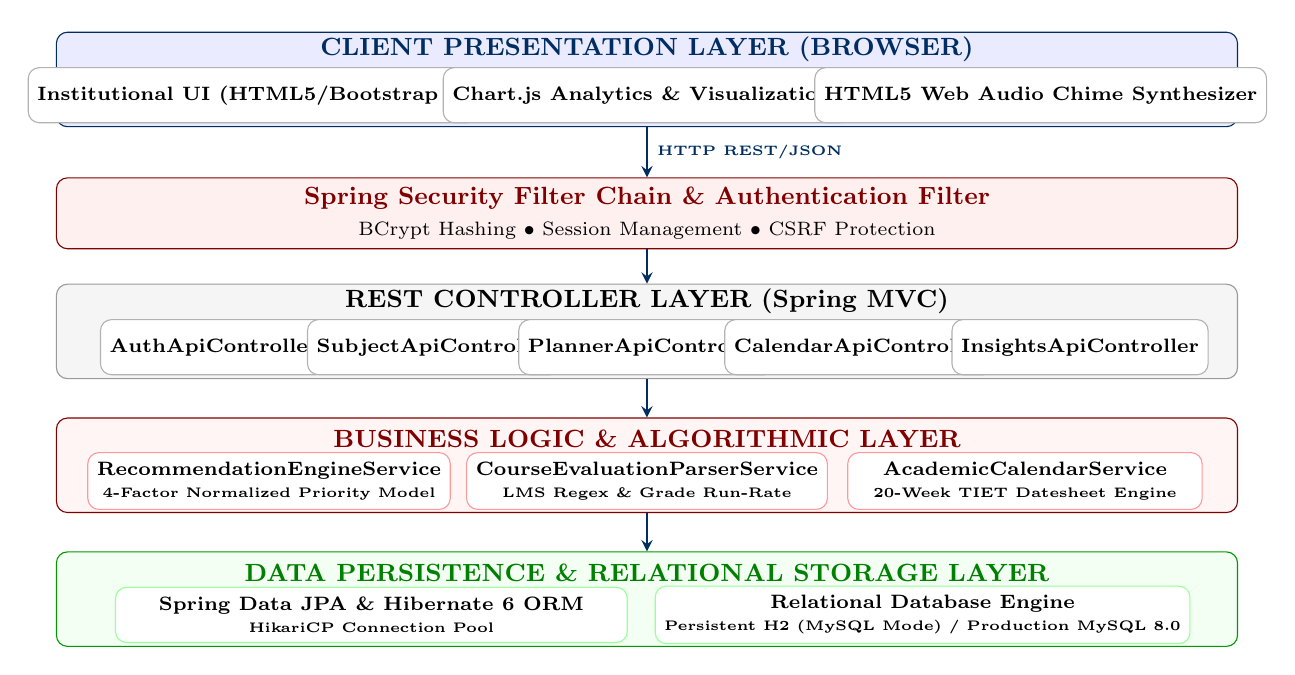
\begin{tikzpicture}[
    layer/.style={rectangle, draw=ThaparNavy, fill=blue!5, rounded corners, minimum width=15cm, minimum height=1.2cm, align=center, font=\small},
    subbox/.style={rectangle, draw=gray!60, fill=white, rounded corners, minimum width=4.4cm, minimum height=0.7cm, font=\scriptsize\bfseries, align=center},
    arrow/.style={thick, ->, >=stealth, color=ThaparNavy}
]
    % Layer 1: Client
    \node[layer, fill=blue!8, draw=ThaparNavy] (client) at (0, 6.0) {};
    \node[above=0.1cm of client.center, font=\bfseries\small\color{ThaparNavy}] {CLIENT PRESENTATION LAYER (BROWSER)};
    \node[subbox] at (-5.0, 5.8) {Institutional UI (HTML5/Bootstrap 5)};
    \node[subbox] at (0, 5.8) {Chart.js Analytics \& Visualizations};
    \node[subbox] at (5.0, 5.8) {HTML5 Web Audio Chime Synthesizer};

    % Layer 2: Security
    \node[layer, minimum height=0.9cm, fill=red!6, draw=ThaparCrimson] (sec) at (0, 4.3) {\textbf{\color{ThaparCrimson} Spring Security Filter Chain \& Authentication Filter}\\ \scriptsize BCrypt Hashing $\bullet$ Session Management $\bullet$ CSRF Protection};

    % Layer 3: Controllers
    \node[layer, fill=gray!8, draw=gray!80] (ctrl) at (0, 2.8) {};
    \node[above=0.1cm of ctrl.center, font=\bfseries\small\color{black}] {REST CONTROLLER LAYER (Spring MVC)};
    \node[subbox, minimum width=2.6cm] at (-5.5, 2.6) {AuthApiController};
    \node[subbox, minimum width=2.6cm] at (-2.7, 2.6) {SubjectApiController};
    \node[subbox, minimum width=2.6cm] at (0, 2.6) {PlannerApiController};
    \node[subbox, minimum width=2.6cm] at (2.7, 2.6) {CalendarApiController};
    \node[subbox, minimum width=2.6cm] at (5.5, 2.6) {InsightsApiController};

    % Layer 4: Services
    \node[layer, fill=red!4, draw=ThaparCrimson] (srv) at (0, 1.1) {};
    \node[above=0.1cm of srv.center, font=\bfseries\small\color{ThaparCrimson}] {BUSINESS LOGIC \& ALGORITHMIC LAYER};
    \node[subbox, minimum width=4.5cm, draw=red!40] at (-4.8, 0.9) {RecommendationEngineService\\ \tiny 4-Factor Normalized Priority Model};
    \node[subbox, minimum width=4.5cm, draw=red!40] at (0, 0.9) {CourseEvaluationParserService\\ \tiny LMS Regex \& Grade Run-Rate};
    \node[subbox, minimum width=4.5cm, draw=red!40] at (4.8, 0.9) {AcademicCalendarService\\ \tiny 20-Week TIET Datesheet Engine};

    % Layer 5: Data
    \node[layer, fill=green!5, draw=green!60!black] (data) at (0, -0.6) {};
    \node[above=0.1cm of data.center, font=\bfseries\small\color{green!50!black}] {DATA PERSISTENCE \& RELATIONAL STORAGE LAYER};
    \node[subbox, minimum width=6.5cm, draw=green!40] at (-3.5, -0.8) {Spring Data JPA \& Hibernate 6 ORM\\ \tiny HikariCP Connection Pool};
    \node[subbox, minimum width=6.5cm, draw=green!40] at (3.5, -0.8) {Relational Database Engine\\ \tiny Persistent H2 (MySQL Mode) / Production MySQL 8.0};

    % Arrows
    \draw[arrow] (client) -- node[right, font=\tiny\bfseries\color{gray}] {HTTP REST/JSON} (sec);
    \draw[arrow] (sec) -- (ctrl);
    \draw[arrow] (ctrl) -- (srv);
    \draw[arrow] (srv) -- (data);
\end{tikzpicture}
\caption{Three-Tier Enterprise System Architecture of Syllabix}
\end{figure}

\newpage
\section{2.2 Use Case Diagram}
The primary actors interacting with the system are the \textbf{Registered Student} and the \textbf{System Automation Engine}.

\vspace{0.4cm}
\begin{figure}[h!]
\centering
\begin{tikzpicture}[
    actor/.style={font=\bfseries\small, align=center},
    usecase/.style={ellipse, draw=ThaparNavy, fill=blue!5, text width=6.5cm, align=center, font=\scriptsize\bfseries, minimum height=0.7cm},
    systembox/.style={rectangle, draw=ThaparCrimson, rounded corners, minimum width=9.5cm, minimum height=11.5cm}
]
    % System Boundary
    \node[systembox] (sys) at (0, 0) {};
    \node[below right=0.2cm of sys.north west, font=\bfseries\color{ThaparCrimson}\small] {Syllabix Academic Platform};

    % Student Actor
    \node[actor] (student) at (-6.5, 0) {
        \begin{tikzpicture}
            \draw[thick, ThaparNavy] (0, 0.7) circle (0.25);
            \draw[thick, ThaparNavy] (0, 0.45) -- (0, -0.15);
            \draw[thick, ThaparNavy] (-0.35, 0.25) -- (0.35, 0.25);
            \draw[thick, ThaparNavy] (0, -0.15) -- (-0.25, -0.6);
            \draw[thick, ThaparNavy] (0, -0.15) -- (0.25, -0.6);
        \end{tikzpicture}\\
        Registered Student\\
        \scriptsize (Jasmine Kaur)
    };

    % Engine Actor
    \node[actor, rectangle, draw=ThaparCrimson, fill=red!5, rounded corners, minimum width=2.0cm, minimum height=1.0cm] (engine) at (6.5, -1.0) {
        $\ll$System$\gg$\\
        Syllabix Core
    };

    % Use Cases
    \node[usecase] (uc1) at (0, 4.8) {UC1: Authenticate / Register / BCrypt Login};
    \node[usecase] (uc2) at (0, 3.8) {UC2: View Academic Dashboard \& Roll Ribbon};
    \node[usecase] (uc3) at (0, 2.8) {UC3: Manage 7 Registered Subjects \& Units};
    \node[usecase] (uc4) at (0, 1.8) {UC4: Extract Syllabus PDF (Apache PDFBox)};
    \node[usecase, draw=ThaparCrimson, fill=red!8] (uc5) at (0, 0.8) {UC5: Paste LMS Scheme \& Calculate Run-Rate};
    \node[usecase] (uc6) at (0, -0.2) {UC6: Track Lab Assignments (Assignments 1-8)};
    \node[usecase] (uc7) at (0, -1.2) {UC7: Consult 20-Week TIET Academic Calendar};
    \node[usecase, draw=ThaparCrimson, fill=red!8] (uc8) at (0, -2.2) {UC8: Generate Adaptive Daily Study Timetable};
    \node[usecase] (uc9) at (0, -3.2) {UC9: Execute Pomodoro Study Session \& Streak};
    \node[usecase] (uc10) at (0, -4.2) {UC10: Simulate What-If CGPA \& Exam Readiness};

    % Associations
    \draw[thick, gray] (student) -- (uc1.west);
    \draw[thick, gray] (student) -- (uc2.west);
    \draw[thick, gray] (student) -- (uc3.west);
    \draw[thick, gray] (student) -- (uc4.west);
    \draw[thick, gray] (student) -- (uc5.west);
    \draw[thick, gray] (student) -- (uc6.west);
    \draw[thick, gray] (student) -- (uc7.west);
    \draw[thick, gray] (student) -- (uc8.west);
    \draw[thick, gray] (student) -- (uc9.west);
    \draw[thick, gray] (student) -- (uc10.west);

    \draw[thick, ThaparCrimson] (uc5.east) -- (engine);
    \draw[thick, ThaparCrimson] (uc8.east) -- (engine);
\end{tikzpicture}
\caption{Use Case Diagram of Syllabix Academic Platform}
\end{figure}

\newpage
\section{2.3 Class Diagram}
The domain model captures all academic entities, their member attributes, operations, and relational multiplicities.

\vspace{0.4cm}
\begin{figure}[h!]
\centering
\begin{tikzpicture}[
    classbox/.style={rectangle, draw=ThaparNavy, fill=white, rounded corners, minimum width=3.4cm, font=\scriptsize, align=left},
    header/.style={fill=ThaparNavy, text=white, font=\scriptsize\bfseries, align=center, minimum width=3.4cm, minimum height=0.45cm},
    redheader/.style={fill=ThaparCrimson, text=white, font=\scriptsize\bfseries, align=center, minimum width=3.4cm, minimum height=0.45cm},
    greenheader/.style={fill=green!40!black, text=white, font=\scriptsize\bfseries, align=center, minimum width=3.4cm, minimum height=0.45cm}
]
    % Student
    \node[classbox] (student) at (-4.8, 3.5) {
        \textbf{Student}\\
        \hline
        - id: Long\\
        - fullName: String\\
        - email: String\\
        - semester: Integer (5)\\
        - dailyHours: Double\\
        \hline
        + register()\\
        + updateHours()
    };

    % Subject
    \node[classbox, draw=ThaparCrimson] (subject) at (0, 3.5) {
        \textbf{Subject}\\
        \hline
        - id: Long\\
        - code: String (UCS553)\\
        - name: String\\
        - credits: Integer (4.0)\\
        - targetGrade: String\\
        \hline
        + getCompletionRate()\\
        + calculateDeficit()
    };

    % Unit
    \node[classbox] (unit) at (4.8, 4.0) {
        \textbf{Unit}\\
        \hline
        - id: Long\\
        - unitNumber: Integer\\
        - title: String\\
        \hline
        + getTopics()
    };

    % Topic
    \node[classbox] (topic) at (4.8, 1.5) {
        \textbf{Topic}\\
        \hline
        - id: Long\\
        - name: String\\
        - difficulty: String\\
        - durationMin: Integer\\
        - isCompleted: Boolean\\
        \hline
        + markComplete()
    };

    % Assessment
    \node[classbox, draw=ThaparCrimson] (assessment) at (-4.8, -0.5) {
        \textbf{Assessment}\\
        \hline
        - id: Long\\
        - title: String (MST)\\
        - type: String\\
        - maxMarks: Double\\
        - date: LocalDateTime\\
        \hline
        + isApproaching()
    };

    % Marks
    \node[classbox, draw=ThaparCrimson] (marks) at (0, -0.5) {
        \textbf{Marks}\\
        \hline
        - id: Long\\
        - marksObtained: Double\\
        - maxMarks: Double\\
        - date: LocalDate\\
        \hline
        + getPercentage()
    };

    % StudyTask
    \node[classbox, draw=green!40!black] (task) at (4.8, -1.0) {
        \textbf{StudyTask}\\
        \hline
        - id: Long\\
        - scheduledDate: LocalDate\\
        - durationMin: Integer\\
        - priorityScore: Double\\
        - isCompleted: Boolean\\
        \hline
        + markComplete()
    };

    % Links
    \draw[thick, ThaparNavy] (student) -- node[above, font=\tiny] {1 \quad\quad *} (subject);
    \draw[thick, gray] (subject) -- node[above, font=\tiny] {1 \quad\quad *} (unit);
    \draw[thick, gray] (unit) -- node[right, font=\tiny] {1} node[right, font=\tiny, below=0.8cm] {*} (topic);
    \draw[thick, ThaparCrimson] (student) -- node[left, font=\tiny] {1} node[left, font=\tiny, below=1.2cm] {*} (assessment);
    \draw[thick, ThaparCrimson] (subject) -- node[right, font=\tiny] {1} node[right, font=\tiny, below=1.2cm] {*} (marks);
    \draw[thick, green!40!black] (topic) -- node[right, font=\tiny] {1} node[right, font=\tiny, below=0.8cm] {*} (task);
\end{tikzpicture}
\caption{Domain Model Class Diagram}
\end{figure}

\newpage
\section{2.4 Activity Diagram}
The workflow below illustrates the recommendation and run-rate scheduling process:

\vspace{0.4cm}
\begin{figure}[h!]
\centering
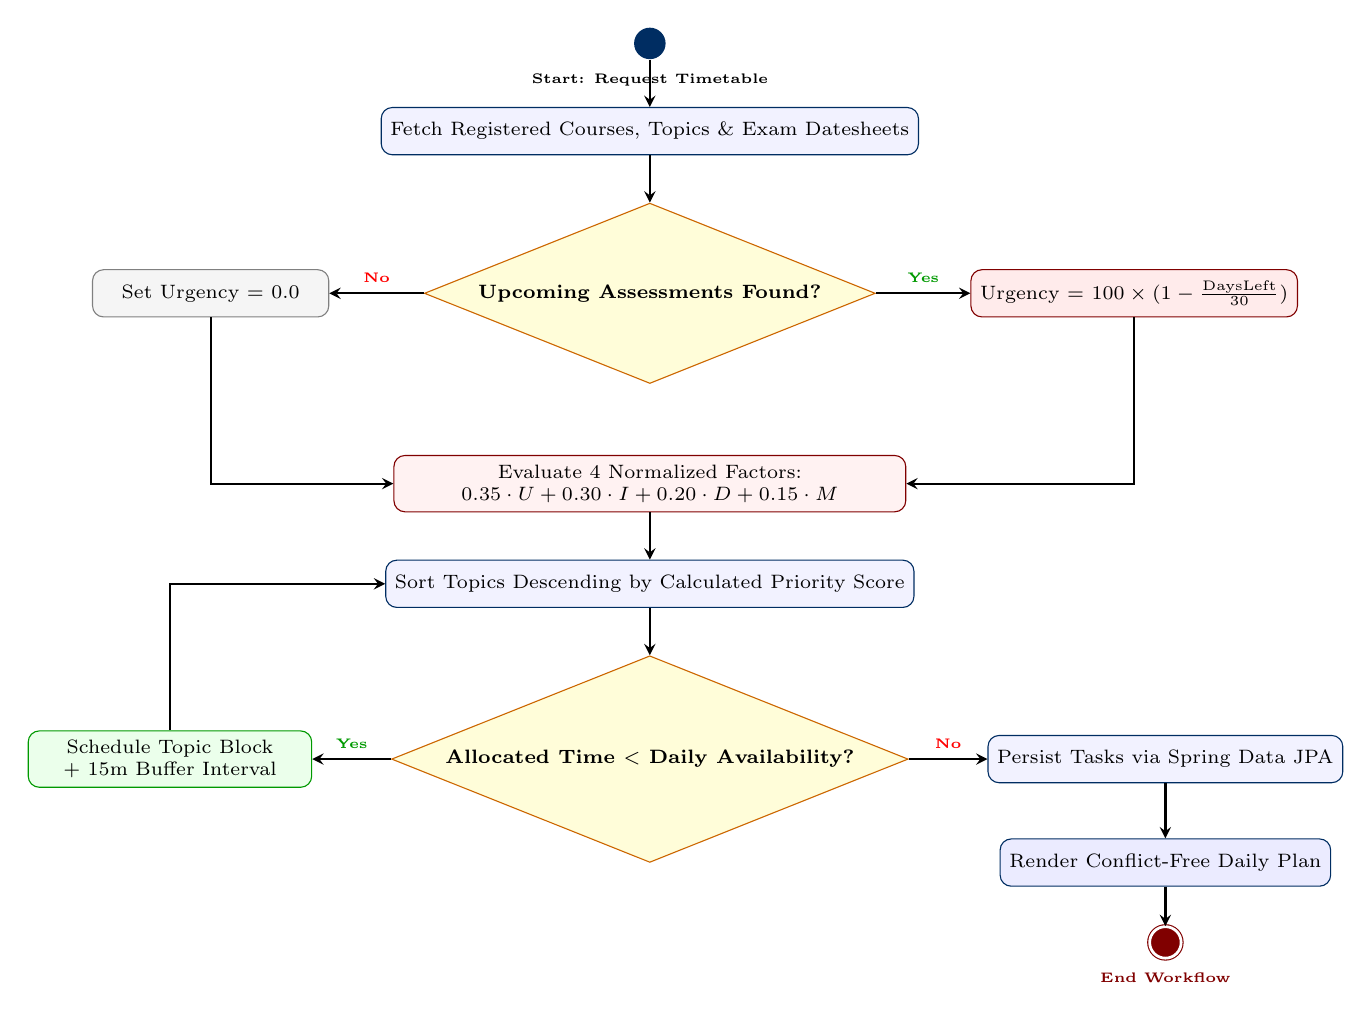
\begin{tikzpicture}[
    node distance=1.1cm,
    stepnode/.style={rectangle, draw=ThaparNavy, fill=blue!5, rounded corners, align=center, font=\scriptsize, minimum width=6.5cm, minimum height=0.6cm},
    decision/.style={diamond, draw=orange!80!black, fill=yellow!15, aspect=2.5, font=\scriptsize\bfseries, align=center},
    point/.style={circle, fill=ThaparNavy, minimum size=0.4cm},
    endpoint/.style={circle, draw=ThaparCrimson, double, double distance=1pt, fill=ThaparCrimson, minimum size=0.4cm},
    arrow/.style={thick, ->, >=stealth}
]
    \node[point] (start) {};
    \node[below=0.05cm of start, font=\tiny\bfseries] {Start: Request Timetable};
    \node[stepnode, below=0.6cm of start] (fetch) {Fetch Registered Courses, Topics \& Exam Datesheets};
    \node[decision, below=0.6cm of fetch] (dec1) {Upcoming Assessments Found?};
    \node[stepnode, fill=red!8, draw=ThaparCrimson, right=1.2cm of dec1, minimum width=4cm] (urgency) {Urgency = $100 \times (1 - \frac{\text{DaysLeft}}{30})$};
    \node[stepnode, fill=gray!8, draw=gray, left=1.2cm of dec1, minimum width=3cm] (nourgency) {Set Urgency = 0.0};
    \node[stepnode, fill=red!5, draw=ThaparCrimson, below=0.9cm of dec1] (weights) {Evaluate 4 Normalized Factors:\\$0.35 \cdot U + 0.30 \cdot I + 0.20 \cdot D + 0.15 \cdot M$};
    \node[stepnode, below=0.6cm of weights] (sort) {Sort Topics Descending by Calculated Priority Score};
    \node[decision, below=0.6cm of sort] (dec2) {Allocated Time $<$ Daily Availability?};
    \node[stepnode, fill=green!8, draw=green!60!black, left=1.0cm of dec2, minimum width=3.6cm] (schedule) {Schedule Topic Block\\+ 15m Buffer Interval};
    \node[stepnode, right=1.0cm of dec2, minimum width=4.0cm] (persist) {Persist Tasks via Spring Data JPA};
    \node[stepnode, fill=blue!8, below=0.7cm of persist, minimum width=4.0cm] (render) {Render Conflict-Free Daily Plan};
    \node[endpoint, below=0.5cm of render] (end) {};
    \node[below=0.05cm of end, font=\tiny\bfseries\color{ThaparCrimson}] {End Workflow};

    \draw[arrow] (start) -- (fetch);
    \draw[arrow] (fetch) -- (dec1);
    \draw[arrow] (dec1) -- node[above, font=\tiny\bfseries\color{green!60!black}] {Yes} (urgency);
    \draw[arrow] (dec1) -- node[above, font=\tiny\bfseries\color{red}] {No} (nourgency);
    \draw[arrow] (urgency) |- (weights);
    \draw[arrow] (nourgency) |- (weights);
    \draw[arrow] (weights) -- (sort);
    \draw[arrow] (sort) -- (dec2);
    \draw[arrow] (dec2) -- node[above, font=\tiny\bfseries\color{green!60!black}] {Yes} (schedule);
    \draw[arrow] (schedule) |- (sort);
    \draw[arrow] (dec2) -- node[above, font=\tiny\bfseries\color{red}] {No} (persist);
    \draw[arrow] (persist) -- (render);
    \draw[arrow] (render) -- (end);
\end{tikzpicture}
\caption{Activity Flowchart of Recommendation \& Run-Rate Engine}
\end{figure}

\newpage
\section{2.5 Database Design / Entity-Relationship (ER) Diagram}
The relational database schema is structured into 8 primary entities managed by Spring Data JPA and Hibernate in MySQL mode:

\vspace{0.4cm}
\begin{figure}[h!]
\centering
\begin{tikzpicture}[
    erbox/.style={rectangle, draw=ThaparNavy, fill=white, rounded corners, minimum width=3.4cm, font=\tiny, align=left},
    header/.style={fill=ThaparNavy, text=white, font=\scriptsize\bfseries, align=center, minimum width=3.4cm}
]
    % STUDENTS
    \node[erbox] (students) at (-5.0, 3.0) {
        \textbf{STUDENTS}\\
        \hline
        \textbf{id : BIGINT [PK]}\\
        full\_name : VARCHAR\\
        email : VARCHAR [UK]\\
        password : VARCHAR (BCrypt)\\
        branch : VARCHAR (COE)\\
        semester : INT (5)\\
        daily\_study\_hours : DOUBLE
    };

    % SUBJECTS
    \node[erbox, draw=ThaparCrimson] (subjects) at (0, 3.0) {
        \textbf{SUBJECTS}\\
        \hline
        \textbf{id : BIGINT [PK]}\\
        \color{red}student\_id : BIGINT [FK]\\
        code : VARCHAR (UCS553)\\
        name : VARCHAR\\
        credits : INT (4.0)\\
        target\_grade : VARCHAR\\
        teacher\_name : VARCHAR
    };

    % UNITS
    \node[erbox] (units) at (5.0, 3.5) {
        \textbf{UNITS}\\
        \hline
        \textbf{id : BIGINT [PK]}\\
        \color{red}subject\_id : BIGINT [FK]\\
        unit\_number : INT\\
        title : VARCHAR
    };

    % TOPICS
    \node[erbox] (topics) at (5.0, 1.2) {
        \textbf{TOPICS}\\
        \hline
        \textbf{id : BIGINT [PK]}\\
        \color{red}unit\_id : BIGINT [FK]\\
        \color{red}subject\_id : BIGINT [FK]\\
        name : VARCHAR\\
        difficulty : VARCHAR\\
        duration\_min : INT\\
        is\_completed : BOOLEAN
    };

    % ASSESSMENTS
    \node[erbox, draw=ThaparCrimson] (assessments) at (-5.0, -1.2) {
        \textbf{ASSESSMENTS}\\
        \hline
        \textbf{id : BIGINT [PK]}\\
        \color{red}subject\_id : BIGINT [FK]\\
        \color{red}student\_id : BIGINT [FK]\\
        title : VARCHAR (MST)\\
        max\_marks : DOUBLE\\
        assessment\_date : TIMESTAMP
    };

    % MARKS
    \node[erbox, draw=ThaparCrimson] (marks) at (0, -1.2) {
        \textbf{MARKS}\\
        \hline
        \textbf{id : BIGINT [PK]}\\
        \color{red}subject\_id : BIGINT [FK]\\
        \color{red}student\_id : BIGINT [FK]\\
        marks\_obtained : DOUBLE\\
        max\_marks : DOUBLE\\
        assessment\_type : VARCHAR
    };

    % STUDY_TASKS
    \node[erbox, draw=green!40!black] (tasks) at (5.0, -1.2) {
        \textbf{STUDY\_TASKS}\\
        \hline
        \textbf{id : BIGINT [PK]}\\
        \color{red}student\_id : BIGINT [FK]\\
        \color{red}topic\_id : BIGINT [FK]\\
        scheduled\_date : DATE\\
        duration\_min : INT\\
        priority\_score : DOUBLE\\
        is\_completed : BOOLEAN
    };

    % Relational lines
    \draw[thick, ThaparNavy] (students) -- node[above, font=\tiny] {1 \quad\quad $\infty$} (subjects);
    \draw[thick, gray] (subjects) -- node[above, font=\tiny] {1 \quad\quad $\infty$} (units);
    \draw[thick, gray] (units) -- node[right, font=\tiny] {1} node[right, font=\tiny, below=0.6cm] {$\infty$} (topics);
    \draw[thick, ThaparCrimson] (students) -- node[left, font=\tiny] {1} node[left, font=\tiny, below=1.0cm] {$\infty$} (assessments);
    \draw[thick, ThaparCrimson] (subjects) -- node[right, font=\tiny] {1} node[right, font=\tiny, below=1.0cm] {$\infty$} (marks);
    \draw[thick, green!40!black] (topics) -- node[right, font=\tiny] {1} node[right, font=\tiny, below=0.6cm] {$\infty$} (tasks);
\end{tikzpicture}
\caption{Entity-Relationship Schema Diagram}
\end{figure}

\section{2.6 Module Description}
\begin{enumerate}
    \item \textbf{User Authentication \& Session Management Module:} Student registration with duplicate email validation, BCrypt cryptographic hashing for stored credentials, secure cookie session management, and isolated multi-tenant workspace separation.
    \item \textbf{Subject \& Syllabus Management Module:} Full CRUD management for registered courses, credit weights, faculty, target grades, and hierarchical units/topics with auto-calculated completion percentages.
    \item \textbf{Course Evaluation Scheme Auto-Parser \& Target Run-Rate Calculator:} Tokenizes LMS evaluation text, extracts grading components, calculates target grade cutoffs ($A^+, A, B$), and computes required run-rate percentage with feasibility verdicts.
    \item \textbf{Academic Calendar \& Datesheet Management Module:} Real-time detection of active semester week (e.g., Week 17 $\bullet$ Teaching), countdowns to Assessment Week (Week 18) and EST Exams (Weeks 19–20), compensatory Saturday timetables, and gazetted holiday countdowns.
    \item \textbf{Lab Assignments Tracker Module (Assignments 1 to 8):} Tracks laboratory submission status, report completions, and viva readiness.
    \item \textbf{Adaptive Study Recommendation \& Timetable Generator Module:} 4-factor heuristic priority calculator and conflict-free daily scheduling bounded by student-declared daily hours.
    \item \textbf{Focus Study \& Pomodoro Module:} Integrated 25/5-minute Pomodoro timer with Web Audio sound synthesis chimes and habit streak tracking.
    \item \textbf{Academic Performance Analytics \& Simulator Module:} Subject-wise performance radar, score trend tracking, and "What-If" CGPA scenario simulator.
\end{enumerate}

% ------------------------------------------------------------------------------
% CHAPTER 3: IMPLEMENTATION
% ------------------------------------------------------------------------------
\newpage
\chapter{\color{ThaparCrimson} Implementation}

\section{3.1 Technologies and Tools Used}
\begin{itemize}
    \item \textbf{Programming Language:} Java 21 (Amazon Corretto / Eclipse Temurin LTS)
    \item \textbf{Framework:} Spring Boot 3.3.5
    \item \textbf{Modules Used:}
    \begin{itemize}
        \item \texttt{spring-boot-starter-web} (REST APIs \& static template routing)
        \item \texttt{spring-boot-starter-data-jpa} (Hibernate 6 object-relational mapping)
        \item \texttt{spring-boot-starter-security} (BCrypt password encoder, SecurityFilterChain)
        \item \texttt{spring-boot-starter-validation} (JSR-380 Bean Validation)
    \end{itemize}
    \item \textbf{Database Engine:} H2 Database Engine v2.2.224 in persistent file-backed MySQL mode (\texttt{jdbc:h2:file:./data/syllabix\_db;MODE=MySQL}) with zero-code toggle to native MySQL 8.0.
    \item \textbf{Document Processing:} Apache PDFBox 3.0.3 for PDF syllabus extraction.
    \item \textbf{Frontend Architecture:} HTML5, CSS3, Vanilla ES6 JavaScript, Bootstrap 5.3.3, Bootstrap Icons 1.11.3, Chart.js 4.4.1.
    \item \textbf{Testing \& Verification:} JUnit 5, Mockito 5.11, Maven Surefire Plugin 3.2.5.
    \item \textbf{Containerization \& Cloud Hosting:} Docker (Multi-stage build), Render Cloud Hosting (\href{https://syllabix-platform-2.onrender.com}{https://syllabix-platform-2.onrender.com}).
\end{itemize}

\section{3.2 Project Structure / Package Structure}
\begin{lstlisting}[language={},numbers=none]
c:\Users\jasmi\OneDrive\Desktop\java_project
|-- Dockerfile                                 # Multi-stage Docker cloud build
|-- render.yaml                                # Render Blueprint cloud config
|-- pom.xml                                    # Maven dependencies & plugins
|-- src
    |-- main
        |-- java/com/syllabix
            |-- SyllabixApplication.java     # Entry point
            |-- config                       # Security & seed data
            |-- controller                   # REST API controllers
            |-- dto                          # Data Transfer Objects
            |-- entity                       # JPA Domain Entities
            |-- exception                    # Global exception handlers
            |-- repository                   # Spring Data Repositories
            |-- service                      # Algorithmic Services
        |-- resources
            |-- application.properties       # DB & server configuration
            |-- static                       # UI assets (HTML, CSS, JS)
    |-- test                                 # JUnit 5 & Mockito test suite
\end{lstlisting}

\section{3.3 Description of Classes and Interfaces}
\begin{itemize}
    \item \textbf{\texttt{RecommendationEngineService.java}:} Implements the normalized 4-factor heuristic priority equation (Urgency, Incompletion, Difficulty, Marks Deficit).
    \item \textbf{\texttt{CourseEvaluationParserService.java}:} Employs regular expressions to parse LMS evaluation descriptions, match recorded marks, calculate target cutoffs, and evaluate run-rate percentages.
    \item \textbf{\texttt{AcademicCalendarService.java}:} Maintains the 20-week date ranges for TIET ODD SEM 2026-27, providing dynamic calculation of the active semester week and distance to milestones.
    \item \textbf{\texttt{SecurityConfig.java}:} Configures stateless session-backed authentication, CSRF exemptions for REST endpoints, and BCrypt bean isolation.
    \item \textbf{\texttt{GlobalExceptionHandler.java}:} Intercepts exceptions and returns structured JSON error responses with proper HTTP status codes.
\end{itemize}

\section{3.4 Implementation of Major Modules}
\subsection{A. Course Evaluation Scheme Parser \& Run-Rate Computation}
When a student inputs an LMS evaluation notice, component patterns identify \texttt{LAB Evaluation}, \texttt{Sessional Quiz}, \texttt{MST}, and \texttt{EST} along with max marks. The service calculates target marks needed, required run-rate percentage, and assigns feasibility verdicts (\textit{ACHIEVABLE}, \textit{STRETCH}, \textit{UNREALISTIC}).

\subsection{B. Academic Calendar Week Calculator}
Using Java's \texttt{LocalDate}, the calendar service maps dates to corresponding semester weeks. For instance, \textbf{November 25, 2026} is evaluated as:
\begin{itemize}
    \item \textbf{Week 17: Teaching} (23 Nov – 28 Nov 2026).
    \item Followed immediately by \textbf{Week 18: Lab Evaluations} (30 Nov – 05 Dec 2026).
    \item Followed by \textbf{Weeks 19–20: EST Examinations} (07 Dec – 19 Dec 2026).
\end{itemize}

\section{3.5 Exception Handling}
The platform implements centralized exception handling using \texttt{@RestControllerAdvice}, gracefully handling \texttt{ResourceNotFoundException} (404), \texttt{MethodArgumentNotValidException} (400), and \texttt{AuthenticationException} (401).

\section{3.6 Collection Framework Usage}
The Java Collections Framework is utilized extensively throughout the business logic: \texttt{List<T>} and \texttt{ArrayList<T>} for ordered entities, \texttt{Map<String, Double>} for availability mapping, and the Java 8+ Streams API (\texttt{filter}, \texttt{map}, \texttt{sorted}, \texttt{collect}) for the recommendation pipeline:
\begin{lstlisting}
List<Topic> rankedTopics = pendingTopics.stream()
    .sorted(Comparator.comparingDouble(t -> -calculatePriorityScore(t, student)))
    .collect(Collectors.toList());
\end{lstlisting}

\section{3.7 Database Connectivity}
Managed through Spring Data JPA over \textbf{HikariCP} (max pool size 10, 30s timeout). The persistent file-backed H2 engine runs in MySQL compatibility mode (\texttt{MODE=MySQL}), ensuring zero-dependency deployment while maintaining native compatibility with MySQL 8.0.

\section{3.8 Important Code Snippets}

\subsection{Snippet 1: The 4-Factor Weighted Priority Algorithm}
\begin{lstlisting}
public double calculateTopicPriorityScore(Topic topic, Student student) {
    // Factor 1: Upcoming Exam Urgency (35%)
    double urgencyScore = calculateExamUrgencyScore(topic.getSubject(), student);
    
    // Factor 2: Syllabus Incompletion (30%)
    double incompletionScore = calculateSyllabusIncompletionScore(topic.getSubject());
    
    // Factor 3: Topic Difficulty (20%)
    double difficultyScore = mapDifficultyToScore(topic.getDifficultyLevel());
    
    // Factor 4: Previous Academic Marks Deficit (15%)
    double performanceDeficitScore = calculatePerformanceDeficitScore(topic.getSubject(), student);
    
    // Weighted Heuristic Summation
    double finalScore = (0.35 * urgencyScore) +
                        (0.30 * incompletionScore) +
                        (0.20 * difficultyScore) +
                        (0.15 * performanceDeficitScore);
                        
    return Math.round(Math.min(100.0, Math.max(0.0, finalScore)) * 10.0) / 10.0;
}
\end{lstlisting}

\subsection{Snippet 2: Target Grade Run-Rate Calculation}
\begin{lstlisting}
double targetCutoff = getCutoffPercentageForGrade(targetGrade);
double neededTotalMarks = dto.getTotalMarks() * (targetCutoff / 100.0);
double marksStillNeeded = Math.max(0.0, neededTotalMarks - scoredSoFar);

double runRate = 0.0;
if (remainingMarks > 0) {
    runRate = (marksStillNeeded / remainingMarks) * 100.0;
}

String feasibility;
if (runRate <= 65.0) {
    feasibility = "ACHIEVABLE";
} else if (runRate <= 85.0) {
    feasibility = "STRETCH";
} else {
    feasibility = "UNREALISTIC";
}
dto.setRequiredRunRatePercentage(Math.round(runRate * 10.0) / 10.0);
dto.setFeasibilityStatus(feasibility);
\end{lstlisting}

% ------------------------------------------------------------------------------
% CHAPTER 4: RESULTS AND SCREENSHOTS
% ------------------------------------------------------------------------------
\newpage
\chapter{\color{ThaparCrimson} Results and Screenshots}

\section{4.1 Main Application Screen}
The main dashboard serves as the central cockpit for student \textbf{Jasmine Kaur (\texttt{102203045})}. It features the formal institutional masthead of Thapar Institute of Engineering \& Technology, the student academic status ribbon indicating Regular standing in Third Year (\texttt{2627ODDSEM}) with 7 enrolled courses (25.0 credits), the AI recommendation directive, the LMS evaluation run-rate calculator, and the lab tracker.

\section{4.2 Functional Screenshots \& Live Outputs}

\subsection{1. Thapar LMS Authentication Portal (\texttt{/login})}
Recreation of the Thapar LMS login interface with academic notice advisory for \texttt{2627ODDSEM} and 1-Click quick login for Jasmine Kaur.
\begin{lstlisting}[language={},numbers=none]
[THAPAR-LMS + Syllabix AI]
Notice: Third-Year curriculum (2627ODDSEM) course registrations and continuous evaluation
Pre-fill: jkaur_be24@thapar.edu | password123
\end{lstlisting}

\subsection{2. Institutional Dashboard \& Course Evaluation Run-Rate (\texttt{/})}
Evaluation Parser Output for \texttt{UCS553} (Enterprise Web Application):
\begin{itemize}
    \item \textbf{Parsed Components:} LAB Evaluation: 20 Marks (Week 18), Sessional Quiz: 10 Marks (Week 12), MST: 30 Marks, EST: 40 Marks
    \item \textbf{Current Scored Marks:} 23.5 / 25.0
    \item \textbf{Remaining Marks Available:} 75.0 Marks
    \item \textbf{Target Grade A (Cutoff $\ge$ 80\%):} Requires 56.5 marks out of remaining 75.0 marks.
    \item \textbf{Required Run-Rate:} \textbf{75.3\%} $\rightarrow$ \textbf{STRETCH (Achievable with consistent preparation)}
\end{itemize}

\subsection{3. Course Catalog \& Registered Curriculum (\texttt{/subjects})}
Displays all 7 Third-Year subjects with credit badges, faculty names, and syllabus progress bars:

\vspace{0.2cm}
\begin{table}[h!]
\centering
\begin{tabularx}{\textwidth}{|c|X|c|X|c|}
\hline
\rowcolor{CodeBorder}
\textbf{Course Code} & \textbf{Course Title} & \textbf{Credits} & \textbf{Course Coordinator} & \textbf{Completion} \\ \hline
\texttt{UCS510} & Computer Architecture and Organization & 4.0 & Dr. Rajesh Kumar & 45\% \\ \hline
\texttt{UCS553} & Enterprise Web Application & 4.0 & Prof. Vivek Sharma & 60\% \\ \hline
\texttt{UCS421} & Ethics and Risk Mitigation in Computing & 2.0 & Dr. Meenakshi Sood & 75\% \\ \hline
\texttt{UCS548} & Foundations of Data Science & 4.0 & Dr. Anupam Garg & 70\% \\ \hline
\texttt{UCS615} & Image Processing & 3.0 & Dr. Harpreet Kaur & 50\% \\ \hline
\texttt{UML501} & Machine Learning & 4.0 & Dr. Neeraj Kumar & 50\% \\ \hline
\texttt{UCS503} & Software Engineering & 4.0 & Prof. Sanjeev Sofat & 60\% \\ \hline
\end{tabularx}
\end{table}

\subsection{4. Official 20-Week Thapar Academic Calendar (\texttt{/calendar})}
Features the 20-Week Semester Strip auto-highlighting \textbf{Week 17 (Current $\bullet$ 23–28 Nov 2026)}, Datesheet Milestones (MST Exams, Diwali Break, Lab Evaluations, EST Exams, Answer Sheet Review), and Gazetted Holidays with live countdowns.

\section{4.3 Input and Output Demonstrations}

\begin{table}[h!]
\centering
\begin{tabularx}{\textwidth}{|X|X|X|}
\hline
\rowcolor{CodeBorder}
\textbf{User Action / Input} & \textbf{System Processing} & \textbf{Displayed Output} \\ \hline
Click \textbf{"Thapar Student"} on Login Screen & Injects credentials \texttt{jkaur\_be24@thapar.edu} \& \texttt{password123} & Fields populated; authenticates with BCrypt; redirects to Dashboard. \\ \hline
Paste raw LMS evaluation text for \texttt{UCS553} & Regex extracts 4 components, checks existing marks & Displays component cards; computes remaining marks (75.0) and required run-rate (75.3\%). \\ \hline
Select date in Academic Calendar & Filters assessments on selected date & Highlights matching events with red (Urgent), orange (Approaching), or green badges. \\ \hline
Click \textbf{"Generate Study Plan"} with 3.5 hrs availability & Priority algorithm ranks pending topics & Schedules 3 targeted study tasks (60m, 60m, 45m) with 15m intervals; leaves 30m buffer. \\ \hline
\end{tabularx}
\end{table}

\section{4.4 Error Handling Demonstrations}

\begin{table}[h!]
\centering
\begin{tabularx}{\textwidth}{|X|X|X|}
\hline
\rowcolor{CodeBorder}
\textbf{Scenario} & \textbf{Input} & \textbf{System Response} \\ \hline
\textbf{Invalid Login Credentials} & Incorrect password & \texttt{HTTP 401 Unauthorized}: "Invalid email or password" toast displayed. \\ \hline
\textbf{Duplicate Course Registration} & Registering \texttt{UCS510} again & \texttt{HTTP 400 Bad Request}: "Subject code UCS510 already registered for this student". \\ \hline
\textbf{Negative Study Duration} & Entering \texttt{-45} minutes & \texttt{HTTP 400 Bad Request}: Validation error "Duration must be greater than 0". \\ \hline
\textbf{Unrealistic Target Run-Rate} & Setting Target Grade $A^+$ when marks already lost & Calculates run-rate $> 100\%$; flags verdict as \textbf{UNREALISTIC} and suggests achievable Grade B. \\ \hline
\end{tabularx}
\end{table}

% ------------------------------------------------------------------------------
% REFERENCES
% ------------------------------------------------------------------------------
\newpage
\begin{thebibliography}{99}
\bibitem{springboot} VMware Tanzu / Broadcom, \textit{Spring Boot Reference Guide (v3.3.5)}, 2024. \url{https://docs.spring.io/spring-boot/}
\bibitem{springsecurity} VMware Tanzu, \textit{Spring Security Core Specification}, 2024. \url{https://docs.spring.io/spring-security/}
\bibitem{hibernate} Red Hat, Inc., \textit{Hibernate ORM 6.5 User Guide}, 2024. \url{https://hibernate.org/orm/documentation/}
\bibitem{pdfbox} The Apache Software Foundation, \textit{Apache PDFBox 3.0.3 API Reference}, 2024. \url{https://pdfbox.apache.org/}
\bibitem{tietcalendar} Office of Dean of Academic Affairs (DoAA), \textit{Official Academic Calendar \& Datesheet for ODD SEMESTER 2026–2027}, Thapar Institute of Engineering \& Technology, Patiala, 2026.
\bibitem{chartjs} Chart.js Authors, \textit{Chart.js HTML5 Canvas Charting Library (v4.4.1)}, 2024. \url{https://www.chartjs.org/}
\bibitem{syllabixrender} Syllabix Cloud Web Service, \textit{Live Production Deployment}, 2026. \url{https://syllabix-platform-2.onrender.com}
\bibitem{syllabixrepo} Syllabix GitHub Repository, \textit{Official Source Code Repository}, 2026. \url{https://github.com/jasminekaur7/syllabix-platform}
\end{thebibliography}

\end{document}
